\documentclass{article}
\usepackage[margin=1in]{geometry}
\usepackage{graphicx}
\usepackage{hyperref,fancyvrb,amsmath}
\usepackage{tikz}

\newcommand{\mydot}[1]{\draw[fill] (#1) circle (0.1);}

\title{Floyd-Warshall Illustration}
\author{Geoffrey Matthews}

\begin{document}

\maketitle

\begin{Verbatim}
for w in Nodes {
  for u in Nodes {
    for v in Nodes {
      if dist[u,v] < dist[u,w] + dist[w,v] {
        dist[u,v] = dist[u,w] + dist[w,v];
        path[u,v] = path[u,w];
      }
    }
  }
\end{Verbatim}

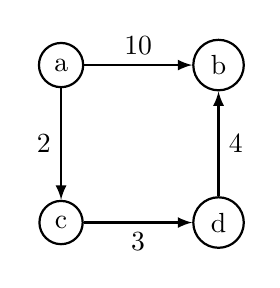
\begin{tikzpicture}[->,>=latex,thick,node distance=2cm]
  \node[draw,circle] (a) {a};
  \node[draw,circle] (b) [right of=a] {b};
  \node[draw,circle] (c) [below of=a] {c};
  \node[draw,circle] (d) [right of=c] {d};
  \draw (a) -- (b) node[midway,above] {10};
  \draw (a) -- (c) node[midway,left] {2};
  \draw (c) -- (d) node[midway,below] {3};
  \draw (d) -- (b) node[midway,right] {4};
\end{tikzpicture}

\begin{tabular}{c|cccc|}
    &a & b& c & d\\\hline
  a & 0 & 10 & 2 & $\infty$ \\
  b & $\infty$ & 0 & $\infty$ & $\infty$\\
  c & $\infty$ & $\infty$ & 0 & 3 \\
  d & $\infty$ & 4 & $\infty$ & 0 \\\hline
  \end{tabular}


\end{document}
